\section{Context}
\subsection{Host organisation}

\medskip

The French Alternative Energies and Atomic Energy Commission (CEA) stands as a cornerstone
of the nation's research landscape. Its multifaceted expertise encompasses a broad spectrum
of fields, including nuclear energy, renewable energy, technological research for industry, material sciences, health and life sciences, and defense and security. The CEA's network
of research centers spans across France, each with its unique specializations and areas
of excellence. Among these, CEA Grenoble holds a prominent position, where I have the 
privilege of pursuing my work-study program. I am part of the labroatory of electrical technology and information (Leti) Institute,
a research center dedicated to microelectronics and nanotechnologies. More specifically, 
I was with “Materials and Structures Properties Laboratory” (MSPL) which is under “Technology Platforms 
Department” (TPFD), one of six different departments of Leti.


\begin{figure}[h!]
    \centering
    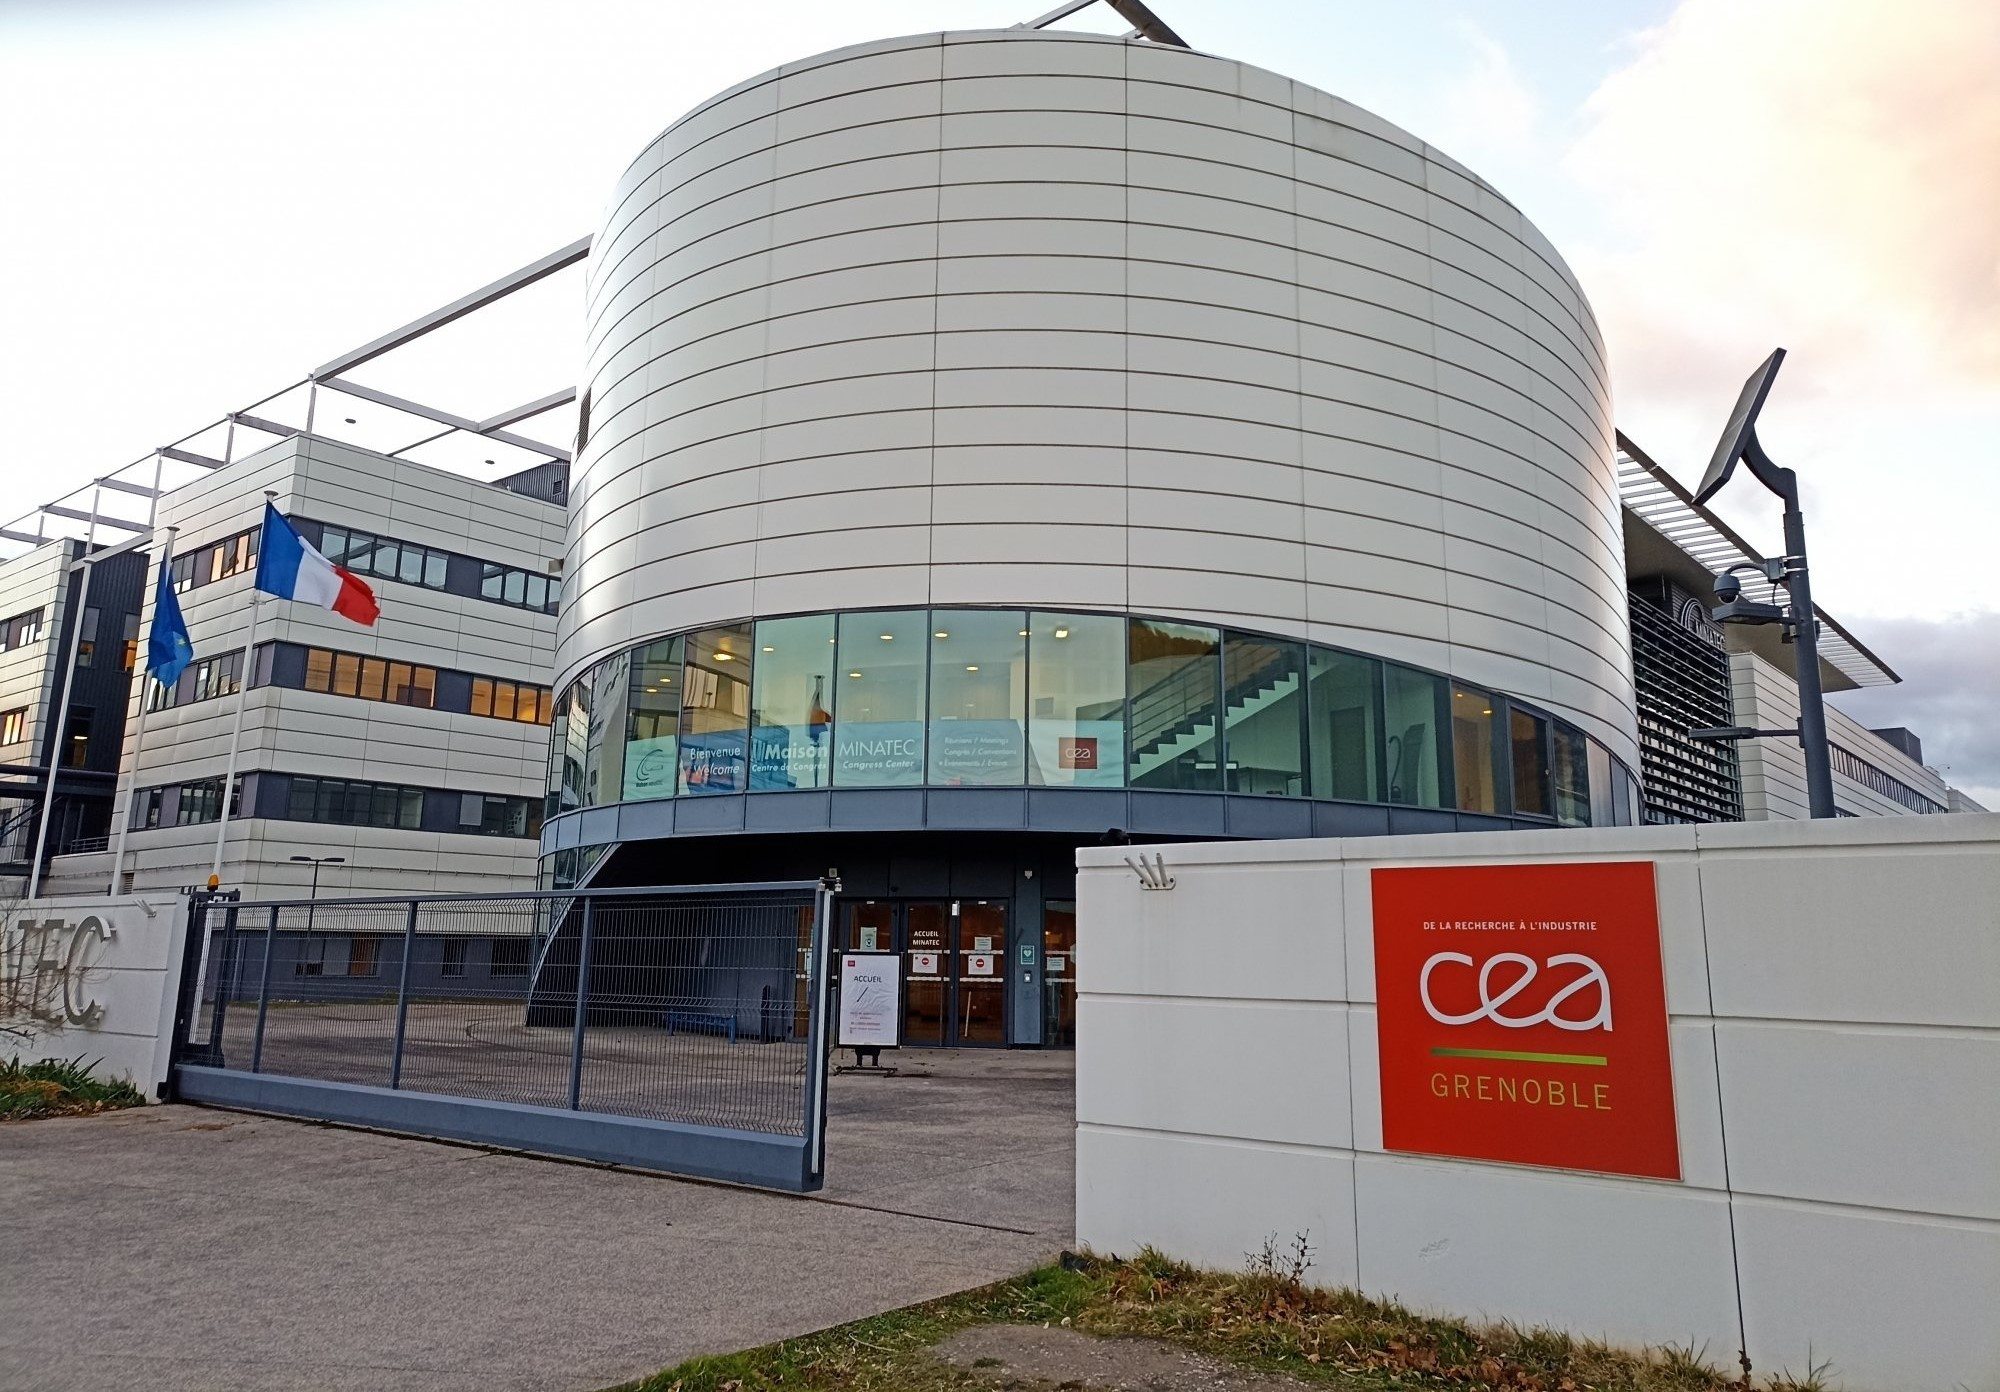
\includegraphics[width=0.8\textwidth]{images/ceaphoto.jpg}
    \caption{CEA Grenoble Campus}
\end{figure}

\FloatBarrier

\subsubsection{History}

\medskip

The French atomic energy commission, CEA, was born in 1945 after World War II. Its mission was to develop nuclear 
expertise for France. Pioneering scientists like Frédéric Joliot-Curie and Francis Perrin led the way in building 
research reactors and nuclear power plants.

\medskip

The CEA didn't stop at just nuclear energy. In the 1960s, they began to diversify into new areas like renewable energy,
 micro and nanotechnologies, defense, and healthcare. This diversification led to the creation of specialized research
 centers, including the future innovation hub, CEA Grenoble.

\medskip

It was founded in 1956 by Nobel laureate physicist Louis Néel. He saw the scientific potential of the Grenoble
region and his vision proved to be true. The center grew rapidly in the following decades, attracting talent and investment
from around the world.

\medskip

It came to be known as France's "atomic capital" due to its research reactors. However, their influence went far beyond
 nuclear. They developed their first integrated circuit in 1965, launching their journey into micro and nanotechnologies. 
 They also played a key role in creating Minatec, the first European hub for excellence in this field. In addition, they 
 became a leader in renewable energy research with the Institut national de l'énergie solaire (Ines).
 European synchrotron radiation facility (ESRF) was also established in Grenoble in 1988, further solidifying the city's
 reputation as a scientific hub.
\medskip

Today, it is a research powerhouse with over 2,500 researchers and technicians. Their campus houses specialized
 institutes in various fields, from healthcare to digital technologies. It's also the headquarters for CEA Tech, the
 technological branch of the CEA with over 4,500 researchers across France.

\begin{figure}[h!]
    \centering
    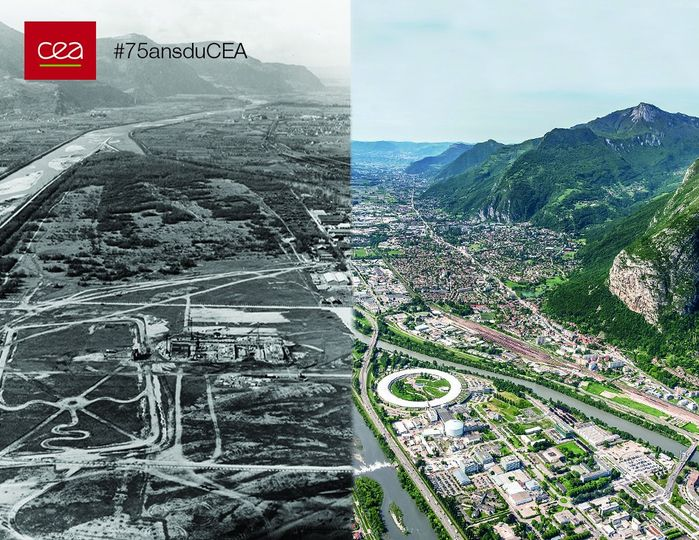
\includegraphics[width=0.8\textwidth]{images/old_new.jpg}
    \caption{CEA Grenoble campus before and after}
\end{figure}

\subsubsection{Sectors of activity}

CEA Grenoble plays a pivotal role in the nation's economic and technological 
advancement through its groundbreaking research and innovations across diverse fields.

\begin{itemize}
  \item \textbf{Energy and Sustainability}: Supporting current and future nuclear power, exploring solar, hydrogen for carbon
   neutrality (2050), researching SMRs (Small modular reactors) and thermonuclear fusion.
  \item \textbf{Digital Technologies}: Contributing through the SPIN program for spintronics (frugal, agile, sustainable computing)
   aligned with France 2030 plan.
  \item \textbf{Healthcare}: Distinguished research in biology and biotechnology for health, addressing current and future challenges.
   (e.g., Laboratoire de biologie et biotechnologie pour la santé)
  \item \textbf{Defense}: Traditionally significant role, developing cutting-edge technologies for national security and defense 
  (less documented for Grenoble).
\end{itemize}

CEA Liten for example also serves as an innovation hub for new energy technologies and nanomaterials, emphasizing energy diversification
 and renewable energy integration. Their research encompasses solar photovoltaics, energy storage, and transportation (hydrogen and fuel
 cells).


\subsubsection{Future and orientation strategy}

\medskip

 CEA stands as a powerhouse for innovation in France.
 Spanning energy, healthcare, defense, and digital technologies, the CEA pushes boundaries by collaborating with universities
 and industry on ambitious R\&D projects.

\medskip

Their focus is clear: develop transformative solutions for global challenges. 
 This includes renewable energy sources, innovative healthcare systems, advanced defense solutions, 
 and disruptive digital technologies. Sustainability is paramount, with research prioritizing energy 
 efficiency and minimizing environmental impact.

\medskip

The CEA partners with leading institutions to accelerate technology transfer and create open innovation ecosystems. 
 These partnerships combine expertise, resources, and networks, leading to breakthrough technologies with significant 
 economic and social value.

\medskip

CEA Grenoble tries to prosper an innovative spirit. They focus on technologies like AI, advanced materials,
 nanotechnologies, and quantum technologies. Their research aims to improve industries, from
 developing next-generation batteries to creating innovative medical devices and advancing digital technologies.

\medskip

The challenges they tackle are various: climate change, the energy transition, emerging diseases, cybersecurity, and 
technological sovereignty. Their research is guided by a long-term vision, anticipating future challenges and preparing 
for them through innovation.

\medskip

The CEA aims to shape a sustainable future. They innovate in clean energy sources, 
advanced healthcare, robust national security, and a cutting-edge digital landscape. By working collaboratively and addressing
 global challenges head-on, the CEA tries to positions itself as a major contributor in the global scientific and technological landscape.

\medskip

\subsection{Project description}

\medskip
CEA Grenoble, a frontrunner in material metrology and characterization, recognizes the potential
 of CD-SAXS for analyzing nanostructures. To this end, CEA has actively invested in CD-SAXS development for several years.

\medskip

During my work-study program, I contributed to this initiative by developing a Python application
 for data fitting and analysis obtained through CD-SAXS. This technique relies on an inverse 
 algorithm that translates scattering intensity data into a relevant real-space structure. The 
 algorithm simulates the experiment using a model and iteratively compares the simulated data 
 with the experimental data until a good fit is achieved. A robust codebase is essential for 
 efficient CD-SAXS data processing.

\medskip

Previously, a collection of functions developed at CEA by former PhD students and at Lawrence Berkeley National Laboratory and Brookhaven National Laboratory served as the 
foundation for CD-SAXS analysis. However, it lacked the coherence of a well-structured application.
The code for various data simulation models was similarly disorganized. My primary task was to 
develop a user-friendly Python application that integrates these functions, streamlining data 
fitting and result analysis.

\medskip

Furthermore, the existing code suffered from slow execution speeds due to a lack of optimisation.
To address this, I implemented optimisations and parallelisation techniques, significantly 
improving the code's efficiency.

\medskip


\subsection{Objectives}

\medskip

The initial aim of this project was commendable - to improve the existing CD-SAXS data analysis 
codebase. However, as we delved deeper, the project's objectives evolved into a series of 
well-defined, targeted enhancements. This iterative approach ensured that our efforts addressed 
the specific needs of researchers at CEA Grenoble.

Here's a breakdown of the key objectives that emerged:

\begin{itemize}
    \item \textbf{Unleashing Computational Power:}
    \begin{itemize}
        \item \textbf{Vectorization for Server Optimization:} Standard code often struggles to fully leverage the parallel processing capabilities of modern servers. We identified the need to vectorize the code, allowing it to efficiently utilize the computational power available on CEA's powerful servers. This significantly boosted the application's overall processing speed.
        \item \textbf{GPU Acceleration - Pushing the Limits:} Recognizing the ever-increasing capabilities of Graphics Processing Units (GPUs), we explored the potential of integrating GPU acceleration into the code. This would potentially unlock even faster performance, enabling us to tackle increasingly complex datasets.
    \end{itemize}
    \item \textbf{User-Centric Design:}
    \begin{itemize}
        \item \textbf{Building a Coherent Application:} The existing code, while functional, lacked the user-friendliness and intuitiveness necessary. We prioritized creating a well-structured, modular application. This would not only simplify data fitting and analysis but also make future feature additions and maintenance easier and more efficient.
        \item \textbf{Addition of different simulation models in the same codebase:} The original codebase had several independant simulation models: a model composed of stacked trapezoid, an overlay model and a rounded trapezoid model. We aimed to integrate these three models into a single, cohesive codebase. This consolidation would streamline the process of selecting and applying different models, enhancing the overall user experience.
      \end{itemize}
    \item \textbf{Quantifying Uncertainty - Confidence in Results:}
    \begin{itemize}
        \item \textbf{MCMC for Uncertainty Estimation:} A critical component missing from the original code was the ability to estimate the uncertainty associated with the fitted parameters. We addressed this by implementing a Markov Chain Monte Carlo (MCMC) algorithm. This powerful technique allowed us to generate a statistically representative set of solutions, enabling us to accurately estimate the level of uncertainty in the fitted parameters.
    \end{itemize}
    \item \textbf{Real-Time Uncertainty Estimation - Saving Valuable Time:}
    \begin{itemize}
        \item \textbf{On-the-Fly Uncertainty:} Taking the concept of uncertainty estimation further, we aimed to integrate this feature into the data acquisition process itself, specifically during synchrotron measurements. This would allow researchers to estimate the uncertainty in real-time. By setting a desired uncertainty threshold, the system could potentially stop the experiment once this level of certainty is achieved. This innovation has the potential to save valuable synchrotron beamtime, a precious resource for researchers.
    \end{itemize}
\end{itemize}

This refined set of objectives ensured that the project delivered valuable enhancements tailored to the needs of CEA researchers. The project not only improved the code's performance but also transformed it into a user-friendly and powerful tool for analyzing CD-SAXS data with greater confidence.
